%-----
% Define o uso do modelo colorido ou preto e branco (escolha uma e descomente)
% Mais abaixo, defina a figura de acordo com a escolha feita.
%-----
%\documentclass{dct-class_bw}
\documentclass{dct-class}

\usepackage{plain}
\begin{document}
\thispagestyle{empty}
%----- As informa��es abaixo s�o obrigat�rias  ----------------------
\titulo{Sem T�tulo Definido}
\autor{Rodrigo Gon�alves de Branco}
\doctipo{Descri��o detalhada do Trabalho}{}
% Observe que a macro doctipo acima tem 2 par�metros
% O primeiro refere-se ao nome do documento
% O segundo � sua identifica��o num�rica, quando ela existir.
% Use a sintaxe \doctipo{XXXXX}{} quando n�o for
% necess�ria a identifica��o num�rica--------------------------------
%--------------------------------------------------------------------
%--------------------------------------------------------------------
%----- As informa��es abaixo s�o opcionais  -------------------------
\orientacao{Prof$^a$. Dr$^a$. D�bora Maria Barroso Paiva}
\docarea{Acessibilidade Digital- Engenharia de Software}
\textofree{}
%-----
% Se voc� usa o latex para compilar, comente as figuras do pdflatex
% Defina a figura do grafo a ser utilizada (escolha uma e descomente)
% Fa�a essa escolha de acordo com a classe escolhida (dct-class_bw ou
% dct-class)
%-----
%\vfill \centerline{\includegraphics[scale=0.8]{logo_dct_bw.mps}}
%\vfill \centerline{\includegraphics[scale=0.8]{logo_dct_color.mps}}
%-----
% Se voc� usa o pdflatex para compilar, comente as figuras do latex
% Defina a figura do grafo a ser utilizada (escolha uma e descomente)
% Fa�a essa escolha de acordo com a classe escolhida (dct-class_bw ou
% dct-class)
%-----
%\vfill \centerline{\includegraphics[scale=0.8]{logo_dct_bw-pdflatex.mps}}
%\vfill \centerline{\includegraphics[scale=0.8]{logo_dct_color-pdflatex.mps}}

\vfill \centerline{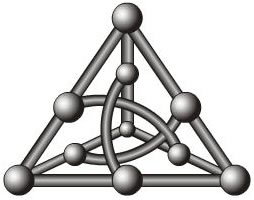
\includegraphics[scale=0.5]{logo_dct.jpg}}

%--------------------------------------------------------------------
% O trecho seguinte n�o pode ser mudado ou retirado -----------------
\vskip 0.5cm
\begin{center}
        Faculdade de Computa��o - FACOM\\
        Universidade Federal de Mato Grosso do Sul\\
        \today
\end{center}
\newpage

\chapter*{Resumo}

Fornecer produtos acess�veis deixou a pouco tempo de ser um diferencial de
determinadas empresas. Acessibilidade, nos dias atuais, � um requisito fundamental de qualquer solu��o desenvolvida, indicando principalmente
respeito e cumplicidade com os clientes. Essa afirma��o � especialmente
verdadeira para os produtos desenvolvidos para a \textit{Internet}, porta de
acesso para toda a intercomunica��o mundial. A \textit{Internet} se mostrou a
tecnologia mais r�pida e barata de aquisi��o de informa��o, levando tecnologias
legadas (servi�os banc�rios, por exemplo) a se adaptarem de forma que pessoas
com dificuldades permanentes ou moment�neas consigam interagir com a sociedade.
Contudo, fornecer um produto acess�vel nem sempre � uma tarefa f�cil. Al�m de
diversas classes diferentes de defici�ncias e dificuldades (o que acarreta
problemas de acessibilidade diferentes), a falta de treinamento e experi�ncia na
�rea faz com que desenvolvedores cometam erros em v�rios aspectos, resultando
num produto inacess�vel. Os modelos de processos e \textit{frameworks} de desenvolvimento de
\textit{software} ainda n�o se adaptaram de forma consistente e homog�nea,
em rela��o a acessibilidade na f�brica de \textit{software}. A �rea de
Tecnologia da Informa��o est� passando por uma fase de transi��o entre o
\textit{HTML 4 e XHTML} para o \textit{HTML 5}, que, entre outras coisas, pretende entregar uma \textit{web} sem�ntica e
tratar dos problemas espec�ficos de acessibilidade, mas que ainda n�o est�
plenamente consolidada. Por fim, as ferramentas dispon�veis aos desenvolvedores
n�o conseguem, de maneira eficaz, auxiliar efetivamente os desenvolvedores a
entregarem um produto acess�vel. Neste trabalho, pretende-se resolver o
problema do escasso suporte ao desenvolvimento de \textit{softwares} acess�veis
presente nas ferramentas de constru��o de \textit{software} dispon�veis,
construindo um \textit{plugin} para o \textit{Eclipse}, uma \textit{IDE
(Integrated Development Environment)} altamente customiz�vel e extens�vel
utilizada por muitos desenvolvedores em todo o mundo.

\label{resumo}
\chapter*{Abstract}

Providing accessible products has recently left  to be a differential
feature of certain companies. Accessibility, today, is a fundamental requirement
of any developed solution, indicating primarily respect and care to
customers.
This statement is especially true for products designed to the Internet which is
the gateway of all  world intercommunication. The Internet has showed to be the
fastest and cheapest technology to acquire information, and has forced legacy
technologies (banking services, for example) to adapt itself so that people with
permanent or momentary difficulties can be able to interact with society.
However, to give an accessible product is not always an easy task. In addition to several different classes of disabilities / difficulties (which leads to
different accessibility problems), lack of training and experience in the area
makes developers producing code in a wrong way, resulting in an inaccessible
product.
The process models and software development frameworks have not been adapted in a
consistent and homogeneous way, contemplating the accessibility in the software
factory. We are going through a transition phase between from the HTML and
XHTML 4 to HTML 5, which among other things, aims to deliver a semantic web and
to treat specific problems of accessibility, but it's not yet fully
consolidated.
Finally, the tools available to developers cannot effectively assist developers to
deliver an affordable product. In this work it is considered that the accessibility requirements should be taken into account during all phases of software development, ie, must evolve from initial requirements analysis to the phase of software testing in order to obtain accessibility as an attribute of software quality of the final product. Thus, we sought primarily to create an approach that could promote accessibility requirements traceability from conception to the coding phase. This approach has associated Requirements, UML models and implementation techniques for accessibility, mapped in an accessibility ontology. In addition, we developed a plugin for Eclipse that promoted the association of technical implementation of accessibility and traceability matrix.

\textbf{Keywords:} \textit{accessibility, requirement traceability,
software development process, CASE tool.}

\label{abstract}

%--------------------------------------------------------------------
% Aqui come�a a inclus�o dos seus textos
%
\renewcommand{\contentsname}{Sum�rio} % renomeando o contentsname
\tableofcontents
%---- O comando abaixo deve ser usado caso queira incluir o conte�do
%como bookmark, visando facilitar a navega��o no Acrobat Reader
%---------------------------------------------------------------------
\addcontentsline{toc}{chapter}{Sum�rio}\label{sumario}
%---------------------------------------------------------------------
%------ Aqui devem ser inclu�dos os cap�tulos ------------------------
\chapter{Introdu��o}

\pagenumbering{arabic}

\setcounter{page}{1}

\section{Contexto e Motiva��o}

A utiliza��o de sistemas para internet � cada vez mais comum. Atividades que
antes eram realizadas presencialmente est�o migrando para servi�os virtuais que
podem ser acessados a partir de qualquer dispositivo com acesso � internet.

A Receita Federal Brasileira, por exemplo, s� recebe as declara��es de Imposto
de Renda via internet \citep{irpf:13}. As declara��es emitidas em
papel foram completamente abandonadas no ano de 2011
\citep{irpf:11}. Essa decis�o foi tomada pois a declara��o feita em papel � mais
vagarosa em todos os aspectos se comparada ao envio da declara��o pela Internet e, al�m disso, era muito grande o n�mero de declara��es preenchidas 
erroneamente usando os formul�rios impressos \citep{irpf_estacao:11}.

Alguns Tribunais j� instituiram a emiss�o de certid�es apenas por meio
eletr�nico. Um exemplo � o Tribunal de Justi�a do Estado do Cear�, que permite a
emiss�o de Certid�o Negativa Criminal por meio de seu \textit{site}
\citep{tjce:11}. Segundo o pr�prio Tribunal, os motivos para adotar a emiss�o de
Certid�o \textit{online} implicam em ``rapidez, transpar�ncia, amplo acesso, interatividade e significativa redu��o
de custos materiais e humanos, contribuindo para os resultados de excel�ncia que
se pretende alcan�ar na presta��o dos servi�os do Judici�rio � popula��o''
\citep{tjce_portaria:11}.

O Conselho Monet�rio Nacional autorizou uma medida que permite que os bancos
possam oferecer aos seus clientes uma conta movimentada exclusivamente por meios
eletr�nicos. Assim, o cliente ficar� isento de cobran�as de tarifas caso fa�a
movimenta��es usando canais eletr�nicos, como Internet, caixas
eletr�nicos e celular \citep{jc:11}.

Os exemplos citados mostram a import�ncia da Internet na dissemina��o de
informa��o e fornecimento de diversos servi�os. A Internet h� muito tempo n�o �
tratada mais como uma ferramenta de luxo ou acess�ria, mas sim como uma
ferramenta essencial nas atividades do cotidiano das pessoas. H� v�rias
vantagens em se usar a Internet para apoiar a comunica��o e os neg�cios das
empresas, por exemplo \citep{oliveira:11}:

\begin{itemize}
  \item Disponibilidade de 24 horas por dia;
  \item Possibilidade de acesso de todas as partes do planeta;
  \item Necessidade de espa�o f�sico e de infra-estrutura reduzidos (ex: bancos)
  para realizar as atividades;
  \item Custo de investimento inicial baixo, etc.
\end{itemize}

Todos deveriam ter pleno acesso aos recursos
fornecidos pela Internet. No entanto, devido a dificuldades e defici�ncias de
determinados grupos de pessoas, o acesso aos recursos pode ficar comprometido,
sendo que em algumas situa��es sequer o acesso � poss�vel. � necess�rio,
portanto, fornecer maneiras de garantir a acessibilidade de informa��es e servi�os da
\textit{Internet}.

\cite{5260918} definem Acessibilidade Digital como o requisito b�sico para
fornecer um acesso equalit�rio � informa��o extra�da da \textit{Internet},
principalmente e especialmente por ser uma maneira vital de acesso ao conte�do
por grupos vulner�veis (principalmente pessoas com necessidades especiais).
Necessidades especiais n�o se referem apenas a pessoas com defici�ncia f�sica
ou mental, mas tamb�m a pessoas com algum tipo de impossibilidade moment�nea,
como a navega��o atrav�s de um \textit{browser} textual ou a visualiza��o de um
\textit{site} atrav�s de um \textit{smartphone}, que possui suas dimens�es reduzidas.

Entregar produtos acess�veis n�o � uma tarefa f�cil. O assunto �
considerado relativamente recente e est� sendo alvo de muitas pesquisas
\citep{lazar:04,brajnik:06,zeng:05}. A acessibilidade na \textit{web} tamb�m j�
� regulamentada em v�rios pa�ses, com diretivas e boas pr�ticas que norteiam sua
aplica��o. Por isso, o papel da Engenharia de \textit{Software} neste contexto �
fundamental. A falta de metodologia e processos bem definidos espec�ficos para acessibilidade podem
gerar produtos n�o acess�veis. Os custos s�o menores quando a
acessibilidade � considerada durante o processo de desenvolvimento do
\textit{software} \citep{groves:11}. Apesar de existir um custo impl�cito
embutido (por exemplo, contrata��o de um especialista em acessibilidade,
ferramentas pr�prias para testes em acessibilidade, etc), em geral, os
benef�cios alcan�ados pela incorpora��o da acessibilidade nos processos s�o
maiores do que os custos envolvidos necess�rios para a entrega do produto,
pois o custo de manuten��o posterior geralmente � mais alto e h� um acr�scimo no
valor agregado ao produto \citep{sherman:01}.

Existem propostas para integrar usabilidade
e acessibilidade aos processos de Engenharia de \textit{Software}
\citep{springerlink:10.1007/978-3-642-02713-0,maia:10}. Outras propostas s�o
espec�ficas para determinadas plataformas \citep{microsoft:09}. Contudo, n�o s�o
encontrados na literatura trabalhos que integram acessibilidade a modelos e
\textit{frameworks} de desenvolvimento bem conhecidos, como \gls{up}
\citep{Jacobson:1999:USD:309683}
(ou sua extens�o mais conhecida
\gls{rup} \citep{rup:13}), \gls{xp}
\citep{Beck:1999:EPE:318762} ou Scrum \citep{DeGrace:1990:WPR:83202}.

T�o importante quanto integrar acessibilidade no processo de desenvolvimento de
\textit{software} s�o as compet�ncias t�cnicas do Engenheiro de
Software, Analista de Sistemas, Projetista e Desenvolvedor.
Devido a fatores como a recente exposi��o do tema nos meios de comunica��o e a defici�ncia no treinamento e forma��o do desenvolvedores,
muitos deles sequer sabem como codificar para tornar seus produtos acess�veis
\citep{1630123, alves:11}. As v�rias classes de problemas de acessibilidade
contribuem para tornar o trabalho de codifica��o ainda mais dif�cil. A utiliza��o de
componentes de \textit{software} com atributos de qualidade embutidos (sistemas
de gerenciamento de conte�do e sistemas \textit{wiki} normalmente possuem um
editor \gls{wysiwyg} que j� s�o acess�veis, como o
\textit{TinyMCE} \citep{tinymce:13}) atenuam mas n�o eliminam o problema. A
conscientiza��o dos desenvolvedores v�m ocorrendo de forma gradual, mas poucas institui��es de ensino brasileiras dedicam uma disciplina espec�fica para Acessibilidade, ou dedicam pouco tempo em disciplinas de �mbito maior como Interface
Humano-Computador, Hiperm�dia/Multim�dia ou Engenharia de \textit{Software}
(Exemplos de grades curriculares:
Harvard\footnote{http://www.seas.harvard.edu/teaching-learning/undergraduate/computer-science/planning-and-courses},
MIT\footnote{http://ocw.mit.edu/courses/electrical-engineering-and-computer-science/\#undergrad},
USP\footnote{http://www.ime.usp.br/dcc/grad/grade},
UFMS\footnote{http://www.sien.ufms.br/cursos/grade/1904} e
IFMS\footnote{http://www.ifms.edu.br/rightsidebar/cursos/graduacao-2/tecnologia-em-sistemas-para-internet/}).

A utiliza��o de ferramentas que ap�iam os profissionais na constru��o de boas
solu��es acess�veis � muito comum, pois aumenta a produtividade, retirando boa
parte do esfor�o necess�rio e diminuindo passos repetitivos que seriam
necess�rios sem o aux�lio de tais ferramentas. Em geral, s�o utilizadas
ferramentas \textit{CASE, IDEs e frameworks}, mas existem algumas ferramentas
espec�ficas para o contexto de acessibilidade. Existem v�rias classes destas
ferramentas espec�ficas, entre elas:

\begin{itemize}
  \item simulador: a ferramenta simula uma defici�ncia/dificuldade, mostrando ao
  desenvolvedor o problema do produto \citep{5358165};
  \item validador: a ferramenta utiliza um conjunto de normas e padr�es
  pr�-definidos e, atrav�s da valida��o objetiva, julga se o produto atende ou
  n�o aos crit�rios definidos\footnote{Exemplo de validador da W3C:
  http://validator.w3.org/};
  \item avaliador: a ferramenta utiliza um validador, complementando com
  informa��es, dicas e m�tricas, al�m de apresentar potenciais problemas que
  devem ser verificados manualmente\footnote{Exemplo de avaliadores:
  Hera(http://www.sidar.org/hera/) e daSilva(http://www.dasilva.org.br/)}.
\end{itemize}

Os avaliadores s�o ferramentas �teis, utilizados para fiscaliza��o e
auditoria de \textit{sites}. Por�m, pesquisas mostram que os desenvolvedores n�o
est�o satisfeitos com os avaliadores dispon�veis
\citep{Trewin:2010:ACT:1805986.1806029}. As ferramentas nem sempre informam de
forma objetiva as mudan�as necess�rias para fornecer um produto acess�vel
\citep{groves:12}. Desenvolvedores iniciantes podem n�o entender as informa��es
apresentadas na ferramenta. E, principalmente, os desenvolvedores est�o
insatisfeitos em utilizar ferramentas externas ao seu ambiente de desenvolvimento
para efetuar a avalia��o \citep{Trewin:2010:ACT:1805986.1806029}.

A situa��o � agravada pela constata��o de que h� poucos estudos que abordam a
engenharia de requisitos e rastreabilidade do ponto de vista do t�pico
acessibilidade, ou seja, poucos estudos t�m indicado como ocorre a evolu��o dos requisitos
de acessibilidade durante o processo de desenvolvimento das aplica��es web \citep{analuizadias:2010}.

\section{Objetivos}

Diante do exposto, os objetivos deste trabalho s�o:

\begin{enumerate}
  \item Estender o \gls{mta} (tratado na se��o \ref{chapter:mta}),
  propondo uma metodologia para a rastreabilidade dos requisitos de acessibilidade
  atrav�s do processo de desenvolvimento de \textit{software};
  \item Permitir a associa��o expl�cita entre os requisitos de
  acessibilidade e os artefatos de documenta��o e, para cada associa��o,
  especificar uma ou mais t�cnicas de implementa��o de acessibilidade de acordo com o documento de conformidade em acessibilidade escolhido;
  \item Implementar uma ferramenta de suporte que seja integrada ao ambiente de
  desenvolvimento e que implemente os objetivos listados acima.
\end{enumerate}

Busca-se identificar pontos de integra��o entre as etapas de engenharia de
requisitos, projeto e implementa��o de c�digo e propor uma ferramenta (\textit{plugin} Eclipse) que represente esta
integra��o. Assim, pretende-se que os requisitos de acessibilidade se tornem
itens de acessibilidade verific�veis e o desenvolvedor dever� ser
informado se a associa��o requisitos, modelos e c�digo est� ou n�o sendo feita. A ferramenta dever�
apresentar sugest�es para que os itens de acessibilidade sejam implementados.
Com isso, pretende-se desenvolver uma ferramenta de apoio � acessibilidade
diferente daquelas apresentadas na literatura, pois ter� como foco a acessibilidade durante o processo de desenvolvimento. 

Com base na pesquisa de \cite{Trewin:2010:ACT:1805986.1806029}, pretende-se que a
ferramenta:

\begin{itemize}
  \item seja orientada ao desenvolvedor (a apresenta��o dos resultados nas
  ferramentas tradicionais s�o adequadas para avalia��o e auditoria de
  \textit{sites}, e n�o para desenvolvedores);
  \item seja integrada ao ambiente de desenvolvimento do desenvolvedor;
  \item apresente informa��es objetivas e no momento em que o desenvolvedor
  desejar visualizar;
  \item tenha rela��o direta entre os requisitos e casos de uso com a etapa de
  codifica��o;
  \item permita que seja feita o rastreamento dos requisitos de acessibilidade,
  desde a sua concep��o at� a fase de codifica��o.
  \item permita que o desenvolvedor consiga verificar, em n�vel de c�digo, a
  associa��o dos requisitos e modelos.
\end{itemize}

\section{Metodologia}

As atividades necess�rias para alcan�ar os objetivos propostos, conforme
mostradas na figura \ref{fig:metodologia} s�o:

\begin{enumerate}
  \item conhecer e definir o escopo do trabalho;
  \item estudar a literatura sobre o assunto;
  \item identificar os pontos de integra��o entre as atividades de engenharia de
  requisitos, projeto e gera��o de c�digo;
  \item estudar o processo de desenvolvimento de \textit{plugins} para o
  \textit{Eclipse};
  \item estudar como t�cnicas de acessibilidade podem ser associadas aos
  modelos \gls{uml};
  \item estudar quais tecnologias existentes podem ser usadas para efetuar a
  associa��o dos requisitos e modelos �s t�cnicas de acessibilidade;
  \item desenvolver a ferramenta;
  \item desenvolver uma prova de conceito, criando um projeto utilizando o
  \gls{mta} e a ferramenta proposta;
  \item apresentar os resultados e conclus�es.
\end{enumerate}

\begin{figure}[h]
\centering
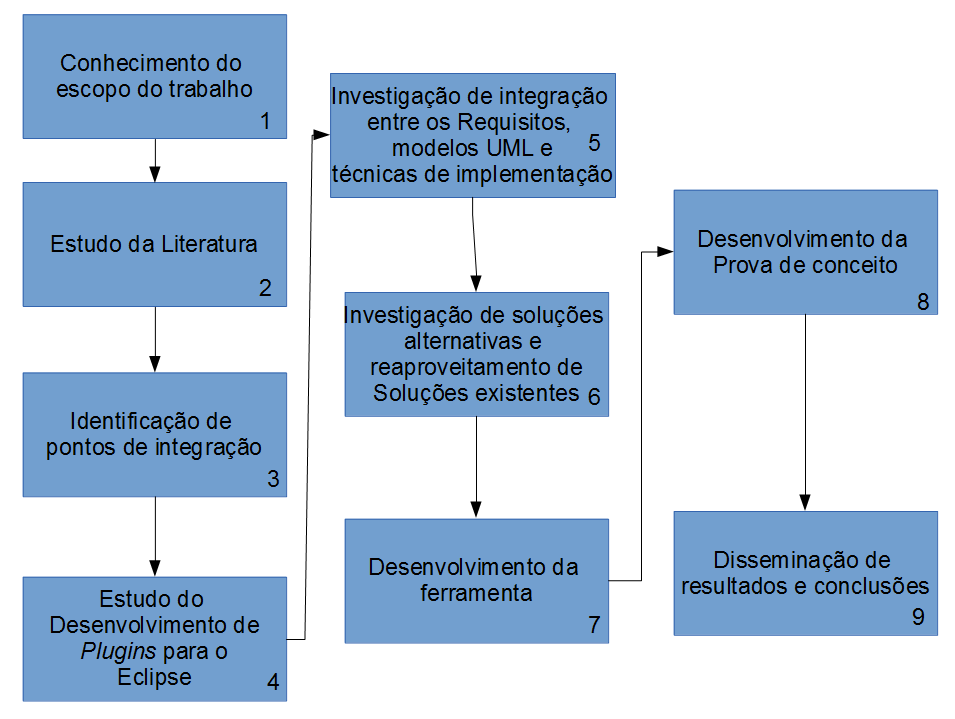
\includegraphics[scale=0.5]{./images/metodologia.png}
\caption{Etapas para a realiza��o deste trabalho}
\label{fig:metodologia}
\end{figure}

\section{Organiza��o do Trabalho}

Este trabalho est� organizado em seis cap�tulos. O primeiro cap�tulo
contextualizou a acessibilidade no desenvolvimento de \textit{sites}, apresentou
alguns desafios conhecidos na �rea e a motiva��o para o desenvolvimento do
mesmo.

O segundo cap�tulo apresenta os detalhes do dom�nio de acessibilidade na
\textit{Internet}. Esse cap�tulo apresenta as tecnologias e conceitos que devem
ser considerados para entregar produtos acess�veis. Tamb�m apresenta as
iniciativas e legisla��es acerca de acessibilidade de produtos \textit{web}.
Por fim, s�o apresentados os principais documentos, refer�ncias e diretrizes
para que os \textit{sites} sejam acess�veis.

O terceiro cap�tulo cont�m o levantamento bibliogr�fico realizado, com breves
descri��es de cada trabalho. O cap�tulo tem por objetivo mostrar qu�o amplo � o
dom�nio de acessibilidade na \textit{Internet}, bem como as propostas sugeridas
e os problemas ainda sem solu��o.

O quarto cap�tulo detalha o processo de integra��o de requisitos de
acessibilidade ao processo de desenvolvimento de \textit{software} (\gls{mta}), apresentando uma ferramenta para demonstrar como a integra��o ocorre.

O quinto cap�tulo apresenta uma prova de conceito, demonstrando a utiliza��o da ferramenta constru�da para a abordagem escolhida, bem como sua efetividade e limita��es.

O sexto e �ltimo cap�tulo apresenta as conclus�es gerais e trabalhos futuros.
%\chapter{Estruturas Utilizadas}

Utilizamos uma \textit{struct} e tr�s classes, s�o elas, respectivamente: \textbf{NodeEdge}, \textbf{Vertex}, \textbf{Graph} e \textbf{Prim}.\\

\section{A \textit{struct NodeEdge}:}
Os objetos desta estrutura representam o peso entre um v�rtice e outro do grafo.\\

\subsection{Suas propriedades:}

\begin{tabular}{|p{0.2\linewidth}|p{0.2\linewidth}|p{0.6\linewidth}|}
\hline
Tipo & Nome & Descri��o\\
\hline
const Vertex* & vertexPt & Aponta para o v�rtice ao qual o est� ligado.\\
\hline
float & weight & Representa o peso da aresta que o liga � vertexPt.\\
\hline
\end{tabular}

\clearpage

\subsection{Seus operadores:}

\begin{tabular}{|p{0.1\linewidth}|p{0.3\linewidth}|p{0.6\linewidth}|}
\hline
Tipo de retorno & Nome & Descri��o\\
\hline
bool & operator$<$(nodeEdge n) & Sobrecarga do operador "menor que", fazendo com que compare o valor da propriedade weight.\\
\hline
bool & operator$>$(nodeEdge n) & Sobrecarga do operador "maior que", fazendo com que compare o valor da propriedade weight.\\
\hline
bool & operator$==$(nodeEdge n) & Sobrecarga do operador "igual a", fazendo com que compare o valor da propriedade weight.\\
\hline
bool & operator$\!=$(nodeEdge n) & Sobrecarga do operador "diferente de", fazendo com que compare o valor da propriedade weight.\\
\hline
bool & operator$>=$(nodeEdge n) & Sobrecarga do operador "maior ou igual a", fazendo com que compare o valor da propriedade weight.\\
\hline
bool & operator$<=$(nodeEdge n) & Sobrecarga do operador "menor ou igual a", fazendo com que compare o valor da propriedade weight.\\
\hline
\end{tabular}

\clearpage

\section{A classe \textit{Vertex}:}
Classe que representa um v�rtice no grafo.\\

\subsection{Seus atributos:}

\begin{tabular}{|p{0.2\linewidth}|p{0.1\linewidth}|p{0.7\linewidth}|}
\hline
Tipo & Nome & Descri��o\\
\hline
char & name[80] & Vetor de 80 posi��es para armazenar o nome do v�rtice.\\
\hline
std::list$<$ NodeEdge $>$ & adj & Lista dos v�rtices adjacentes, com o peso das suas respectivas arestas.\\
\hline
\end{tabular}

\subsection{Seus m�todos:}
\begin{tabular}{|p{0.2\linewidth}|p{0.3\linewidth}|p{0.5\linewidth}|}
\hline
Tipo de retorno & Nome & Descri��o\\
\hline
- & Vertex() & M�todo construtor padr�o, apenas inst�ncia um objeto da classe, sem definir nada.\\
\hline
- & Vertex(const char* nome) & M�todo construtor, que atribui nome ao atributo de classe name.\\
\hline
- & {\Large $\tilde{}$}Vertex() & M�todo destrutor.\\
\hline
void & setName(char* nome) & M�todo que atribui nome ao atributo de classe name.\\
\hline
void & setAdj(Vertex* pt, float w) & M�todo que adiciona pt ao atributo de classe adj.\\
\hline
const std::list$<$ NodeEdge $>$* & getAdj() & M�todo que retorna o atributo de classe adj.\\
\hline
const char* & getName() & M�todo que retorna o valor do atributo de classe name.\\
\hline
float & weight(const char* nome) & M�todo que retorna o peso de uma aresta que incide nesse v�rtice.\\
\hline
\end{tabular}

\clearpage

\section{A classe \textit{Graph}:}
Classe que representa o grafo.\\

\subsection{Seus atributos:}

\begin{tabular}{|p{0.3\linewidth}|p{0.1\linewidth}|p{0.6\linewidth}|}
\hline
Tipo & Nome & Descri��o\\
\hline
std::vector$<$ Vertex $>$ & vert & Vetor com os v�rtices que pertencem ao grafo.\\
\hline
int & current & Atributo necess�rio para o operador de incremento ( operator++ ).\\
\hline
\end{tabular}

\subsection{Seus m�todos:}
\begin{tabular}{|p{0.1\linewidth}|p{0.3\linewidth}|p{0.6\linewidth}|}
\hline
Tipo de retorno & Nome & Descri��o\\
\hline
- & Graph() & M�todo construtor padr�o, apenas inst�ncia um objeto da classe, sem definir nada.\\
\hline
- & Graph(int size) & M�todo construtor, que inicia o grafo alocando size posi��es para o atributo de classe vert.\\
\hline
void & addVertex(const char* nome) & M�todo que adiciona um v�rtice nome ao grafo.\\
\hline
int & searchElement(const char* nome) & M�todo que busca e retorna a posi��o do v�rtice nome no grafo.\\
\hline
bool & addEdge(const char*, const char*, float) & M�todo que adiciona uma aresta ao grafo.\\
\hline
float & weight(const char*, const char*) & M�todo que retorna o peso da aresta que liga os v�rtices cujo nome � passado como par�metro.\\
\hline
const char* & getName() & M�todo que retorna o valor do atributo de classe name.\\
\hline
const Vertex* & operator++ & Sobrecarga do operador incremento, para que ele percorra o vetor de v�rtices.\\
\hline
\end{tabular}

\clearpage

\section{O tipo vecKey:}
Tipo definido para facilitar a refer�ncia a uma estrutura de dados mais complexa.\\
Serve como um "apelido" para std::vector $<$ NodeEdge $>$.\\

\section{A classe \textit{Prim}:}
Classe respons�vel por executar todas as opera��es necess�rias para a utiliza��o do Algoritmo de Prim, bem como o pr�prio algoritmo.\\

\subsection{Seus atributos:}

\begin{tabular}{|p{0.2\linewidth}|p{0.1\linewidth}|p{0.7\linewidth}|}
\hline
Tipo & Nome & Descri��o\\
\hline
vecKey* & fact & Vetor que armazena os v�rtices com peso j� "relaxado".\\
\hline
vecKey* & key & Vetor que armazena os v�rtices com peso "infinito".\\
\hline
Graph* & g & Armazena o grafo.\\
\hline
int & size & N�mero de v�rtices do grafo.\\
\hline
\end{tabular}

\subsection{Seus m�todos:}
\begin{tabular}{|p{0.1\linewidth}|p{0.2\linewidth}|p{0.7\linewidth}|}
\hline
Tipo de retorno & Nome & Descri��o\\
\hline
- & Prim() & M�todo construtor, faz leitura das informa��es, tais como a raiz e o n�mero de v�rtices, al�m de inicializar os atributos da classe.\\
\hline
- & {\Large $\tilde{}$}Prim() & M�todo destrutor, desaloca todas as estruturas utilizadas.\\
\hline
bool & makeGraph() & M�todo que const�i o grafo, fazendo a leitura das informa��es restantes.\\
\hline
float & algoritmPrim() & M�todo que retorna o peso da �rvore geradora m�nima, executando o Algoritmo de Prim.\\
\hline
const Vertex* & extraiMinimo() & M�todo que compara todos os elementos do atributo de classe key, retirando deste atributo o que possuir menor peso, e depois inserindo-o no atributo de classe fact e retornando sua posi��o.\\
\hline
int & searchKey(const char*) & M�todo que retorna a posi��o do v�rtice de nome passado como par�metro, caso n�o encontre, retorna -1.\\
\hline
\end{tabular}
%\chapter{Dificuldades Enfrentadas}

Encontramos certa dificuldade na hora de modelar as estruturas de dados para representar o problema de forma efici�nte.\\
\noindent Resolvemos por utilizar a estrutura de dados \textit{List}, que faz parte da biblioteca padr�o do C++, por ter uma implementa��o otimizada para casos gerais, e ser de f�cil manipula��o ( possui interface rica, com m�todos iteradores e m�todos para inser��o e remo��o de elementos )\\
Tivemos algumas dificuldades na utiliza��o da estrutura List, o que demandou pesquisa, mas acarretou em um bom aprendizado sobre a \textit{STL} ( Standard Template Library ) e a linguagem C++.\\
\noindent Ainda na STL, tivemos alguns problemas na hora de utilizar a fun��o \textit{min\_element}, que foi necess�rio no nosso m�todo Prim::extraiMinimo. Para utiliza-la, tivemos de sobrecarregar os operadores de compara��o da classe NodeEdge.\\
%\chapter{Conclus�o}

Neste trabalhos vimos como a Ci�ncia da Computa��o pode servir de "meio" para que outras �reas do conhecimento cheguem a seu prop�sito.\\

Vimos uma implementa��o do Algoritmo de Prim, que apesar de n�o ser a mais efici�nte dispon�vel, possui um desempenho aceit�vel.\\
Descobrimos novas formas de se representar um grafo computacionalmente, de forma concisa e relativamente efici�nte, al�m de aprofundar na implementa��o usando recursos pr�prios da linguagem C++.
%---------------------------------------------------------------------
% Aqui est� um exemplo de bibliografia
% Veja o arquivo bibi_exemplo.bib
% Para voc� ter um " GUIA "
%---------------------------------------------------------------------
\refstepcounter{chapter}
\refstepcounter{chapter}% Adiciona 1 to chapter ou seja (\thechapter=\thechapter+1)
\addcontentsline{toc}{chapter}{Refer�ncias Bibliogr�ficas}\label{bibliografia}
\nocite{*}

%-----
% Define o estilo das refer�ncias bibliogr�ficas
%-----
%\bibliographystyle{dct-alpha}
%\bibliographystyle{dct-plain}
\bibliographystyle{sbc}
%
\bibliography{sbc-template}
%--------------------------------------------------------------------
\end{document}
